\section{Methods}
\label{sec:ral24_methods}

As this work does not alter the fundamental principles of
\ac{fabrics}, this section focuses on the integration of
three different implicit environment representations into
the framework. In the process, we lay out the necessary
concepts required for the representations, and provide the
tools to combine them with \ac{fabrics}.
%
\subsection{Signed distance fields}
\label{sub:signed_distance_fields}

\paragraph{Representation}
Collision avoidance can be realized using \ac{sdf}
\cite{Oleynikova2017voxblox}.
In this approach, the environment is discretized into a grid and a distance to
the closest obstacle of the environment is assigned to each voxel in the grid.
The distance is zero on the
obstacle's surface and in its inside and positive outside the obstacle.
In \cite{Oleynikova2017voxblox}, the \ac{sdf} is computed
based on Lidar data in combination with continuous mapping,
but other ways to generate \acp{sdf} are possible, see
\cite{Liu2022regularized,Koptev2023neural} for some
manipulation examples.
In this work, we are addressing dynamic environments, so the \ac{sdf} changes
over time, see \cref{fig:sdf} for a two-dimensional example.
%
\begin{figure}[ht]
  \centering
  \begin{subfigure}{0.25\linewidth}
    \centering
    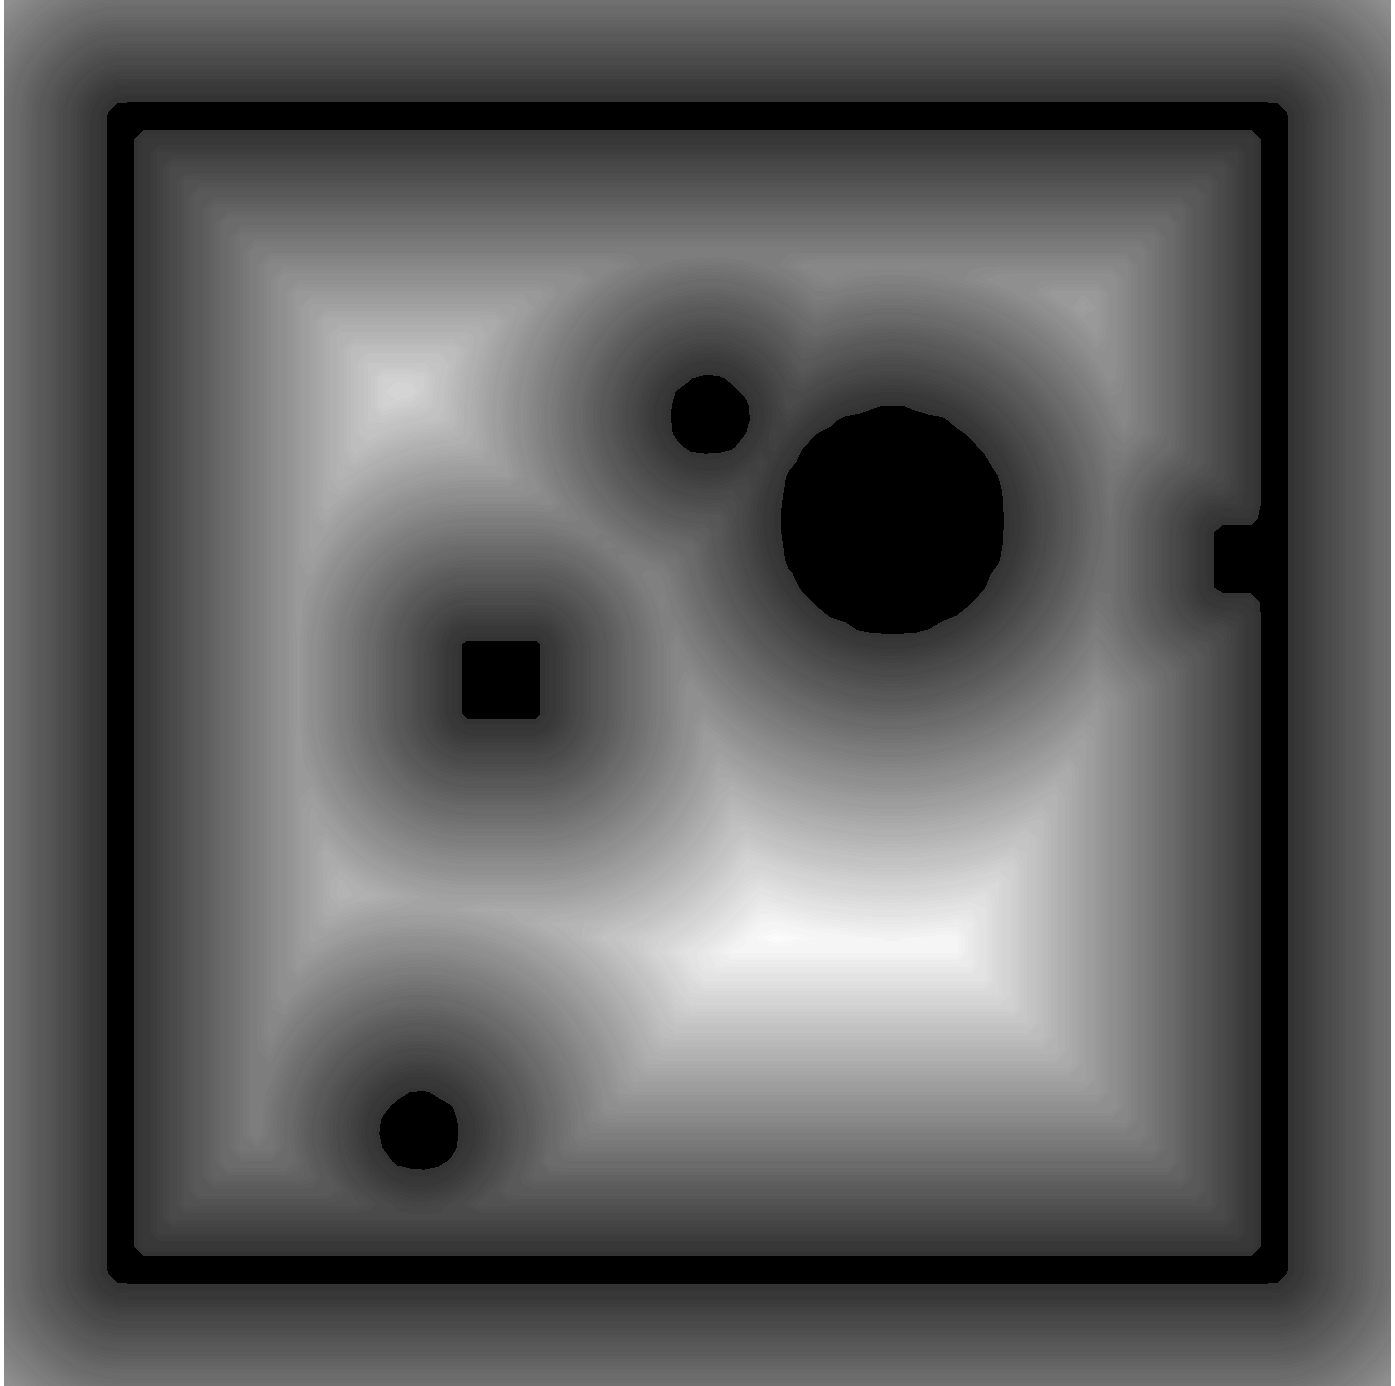
\includegraphics[width=1.00\textwidth]{methods/sdf_1.png}
  \end{subfigure}%
  \begin{subfigure}{0.25\linewidth}
    \centering
    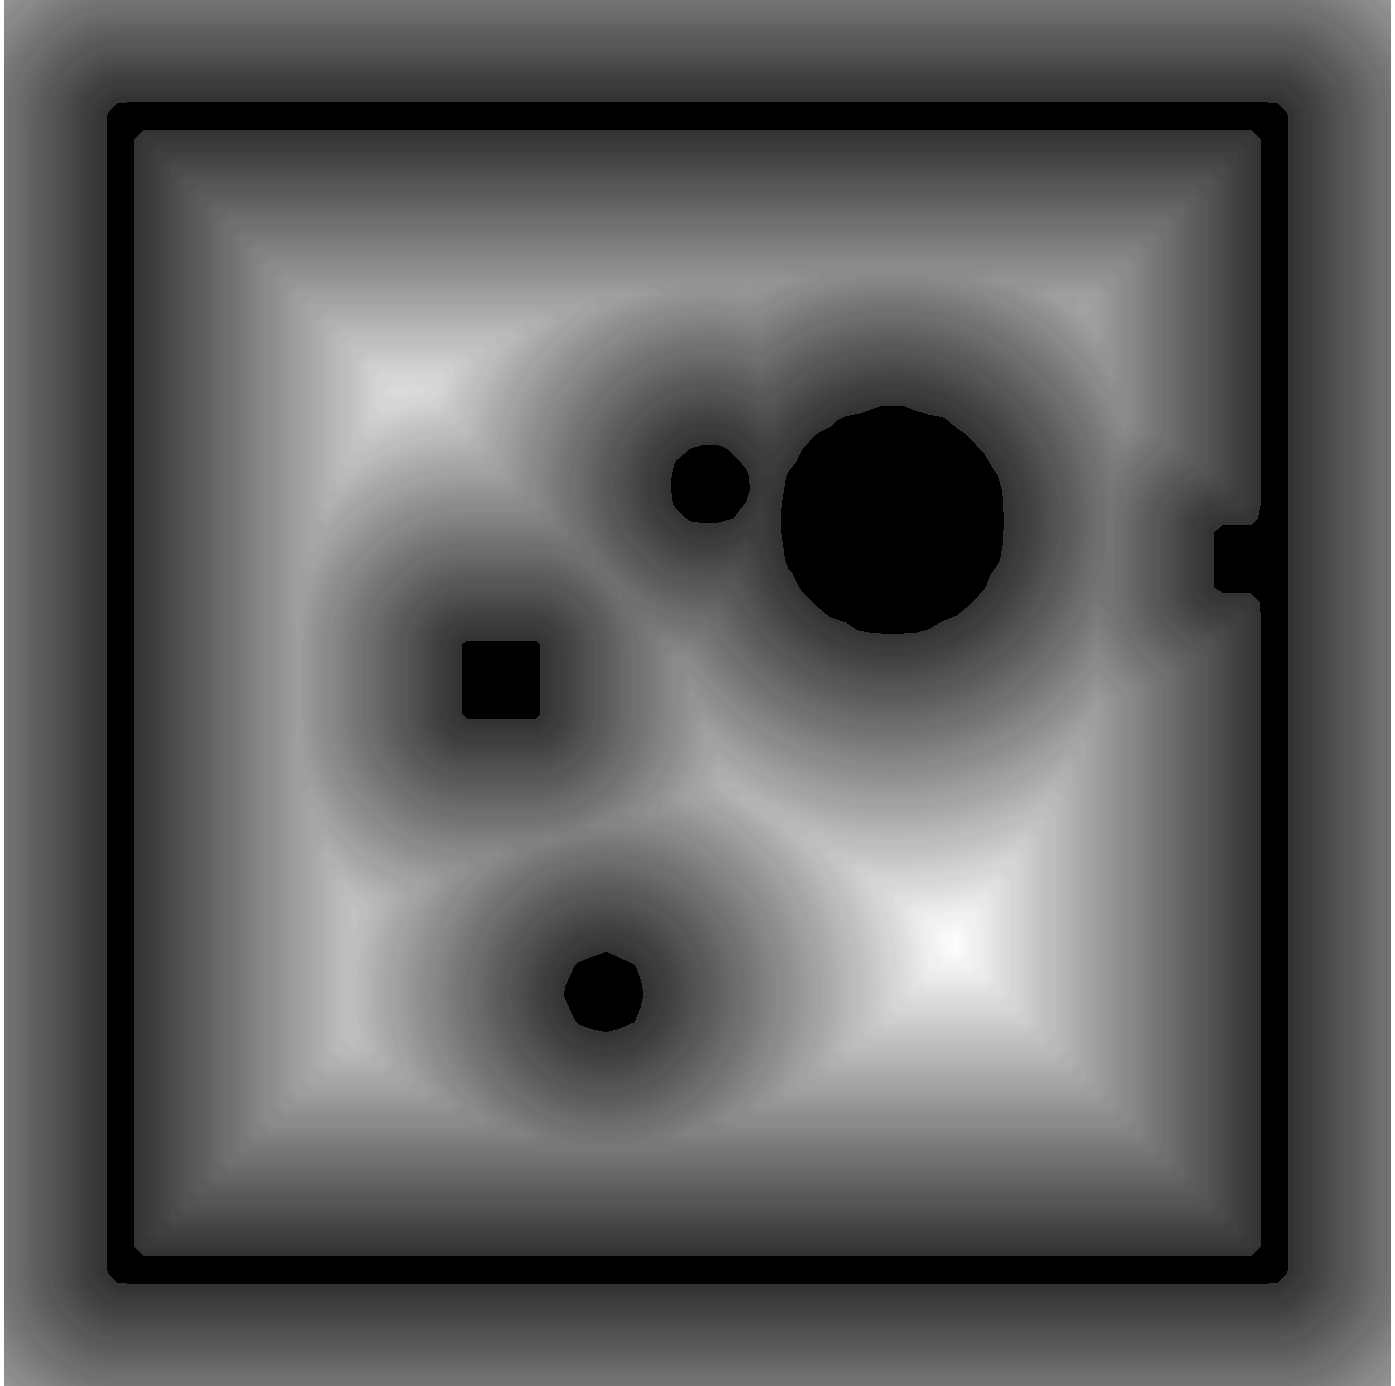
\includegraphics[width=1.00\textwidth]{methods/sdf_2.png}
  \end{subfigure}%
  \begin{subfigure}{0.25\linewidth}
    \centering
    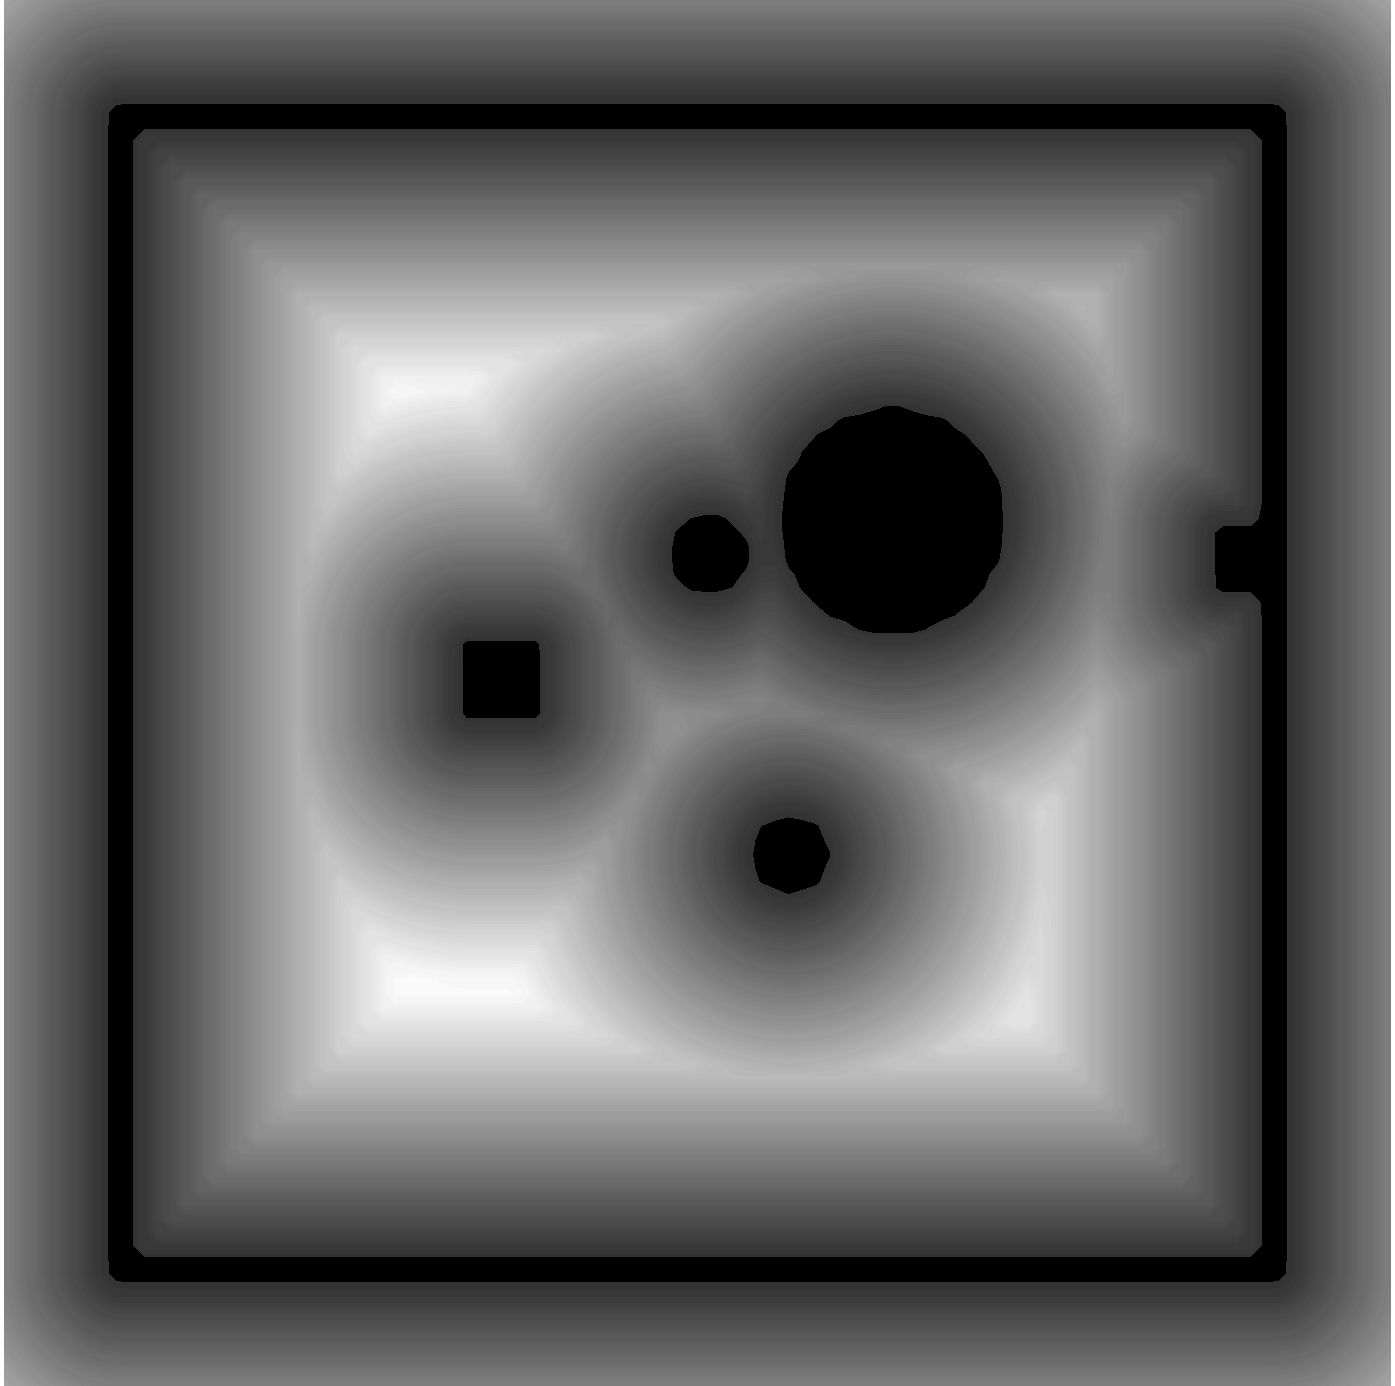
\includegraphics[width=1.00\textwidth]{methods/sdf_3.png}
  \end{subfigure}%
  \begin{subfigure}{0.25\linewidth}
    \centering
    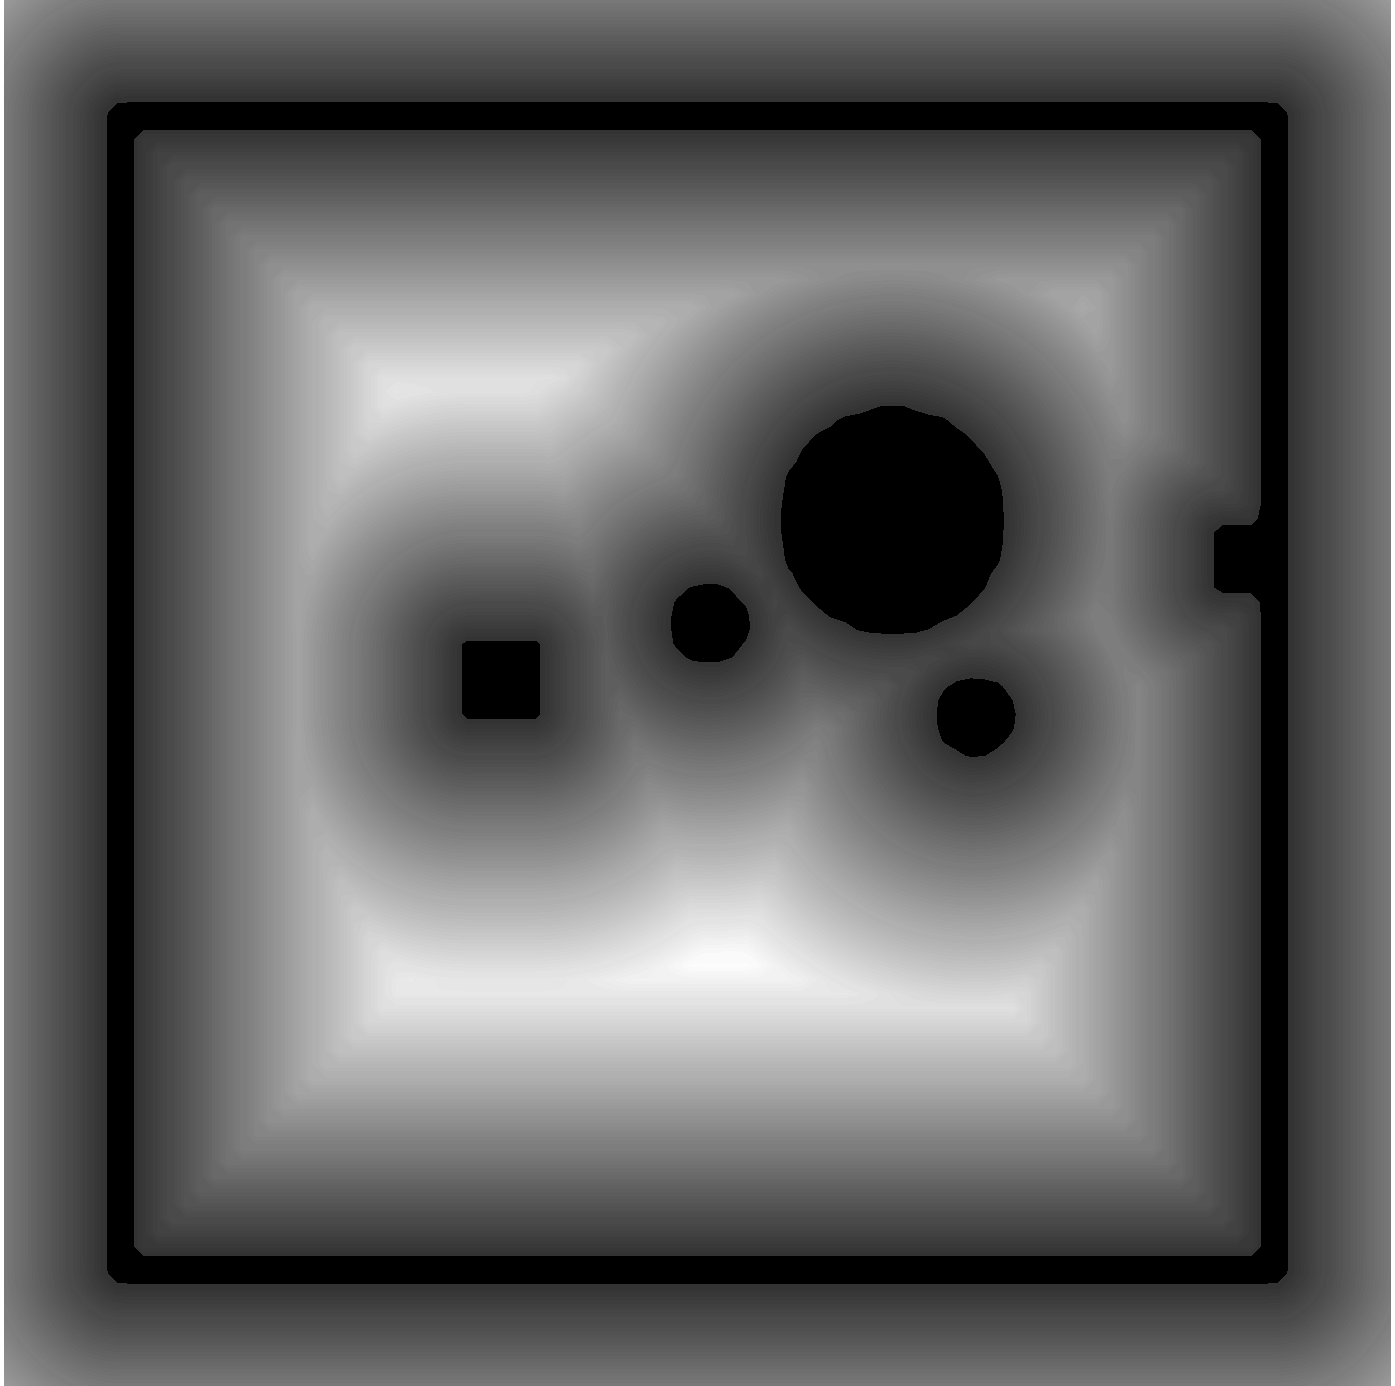
\includegraphics[width=1.00\textwidth]{methods/sdf_4.png}
  \end{subfigure}
  \caption{Changing Signed Distance Field in 2D.
  }%
  \label{fig:sdf}
\end{figure}

%Collision avoidance in the context of \ac{fabrics} is based on
%individual task manifolds for each collision obstacle. The geometry and the 
%weighing Finsler energy are defined in the correpsonding task manifold \X{}.
%To combine those tasks the geometries and the energies are pulled back into the
%root space, usually defined as the configuration space \Q{}.
\paragraph{Integration}
According 
to \cref{eq:pullback}, the integration of collision
avoidance requires the computation of the gradient \J{}.
When the environment is represented as a \ac{sdf}, the gradient cannot be
computed analytically, as it is possible for simple geometric shapes in
\cite{Ratliff2021,Spahn2023}. To overcome this limitation, we propose to
use the numerical gradient as an approximation instead.
The \ac{sdf} is evaluated based on the forward kinematics of the collision link,
so $\map_{sdf}(\fk)$ is a function of \q{}.
As $\der{\q}{\map_{sdf}}$ is not analytically accessible due to the numerical
nature of \acp{sdf}, we apply the chain rule to obtain
\[
  \derf{\q}{\map_{sdf}} = \derf{\fk}{\map_{sdf}}\derf{\q}{\fk}.
\]
The second term $\der{\q}{\fk}$ is the gradient of the forward
kinematics, which can be computed analytically. The first part is the gradient
of the \ac{sdf} which can be
approximated using finite differences:
\[
  \left(\derf{\fk}{\map_{sdf}}\right)_i \approx 
  \frac{\map_{sdf}(\fk + \Delta_i e_i) - \map_{sdf}(\fk - \Delta_i e_i)}{2 \Delta_i},
\]
where $\Delta$ is the resolution in the $i$-th dimension. For 
\ac{fabrics}, the gradient and the value of the \ac{sdf} must be computed externally
at each time step, while the analytical compenent is stored internally. Similar
to \cite{Ratliff2021}, we omit the curvature term \Jdot{} in the pullback
operation.
%
When working with multi-link robots, such as manipulators, different manifolds
are created for the different collision links. Note, that
the same \ac{sdf}
can be used and does not require extra computation.

\subsection{Free space decomposition}
\label{sub:Free Space Decomposition}

\begin{figure}[ht]
  \centering
  \begin{subfigure}{0.33\linewidth}
    \centering
    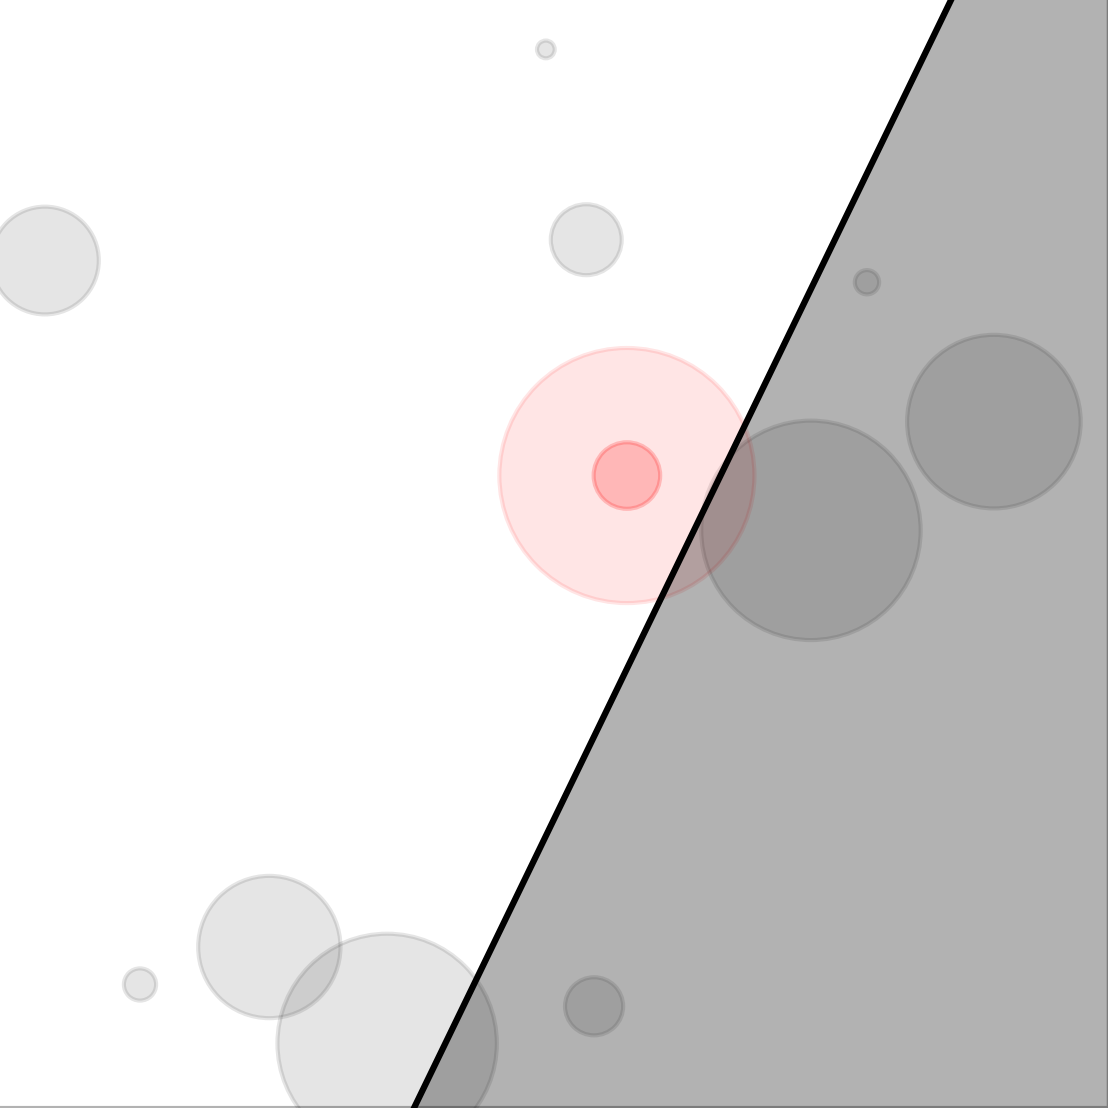
\includegraphics[width=.95\textwidth]{methods/fsd_plot_0.png}
    \vspace*{0.5em}
  \end{subfigure}%
  \begin{subfigure}{0.33\linewidth}
    \centering
    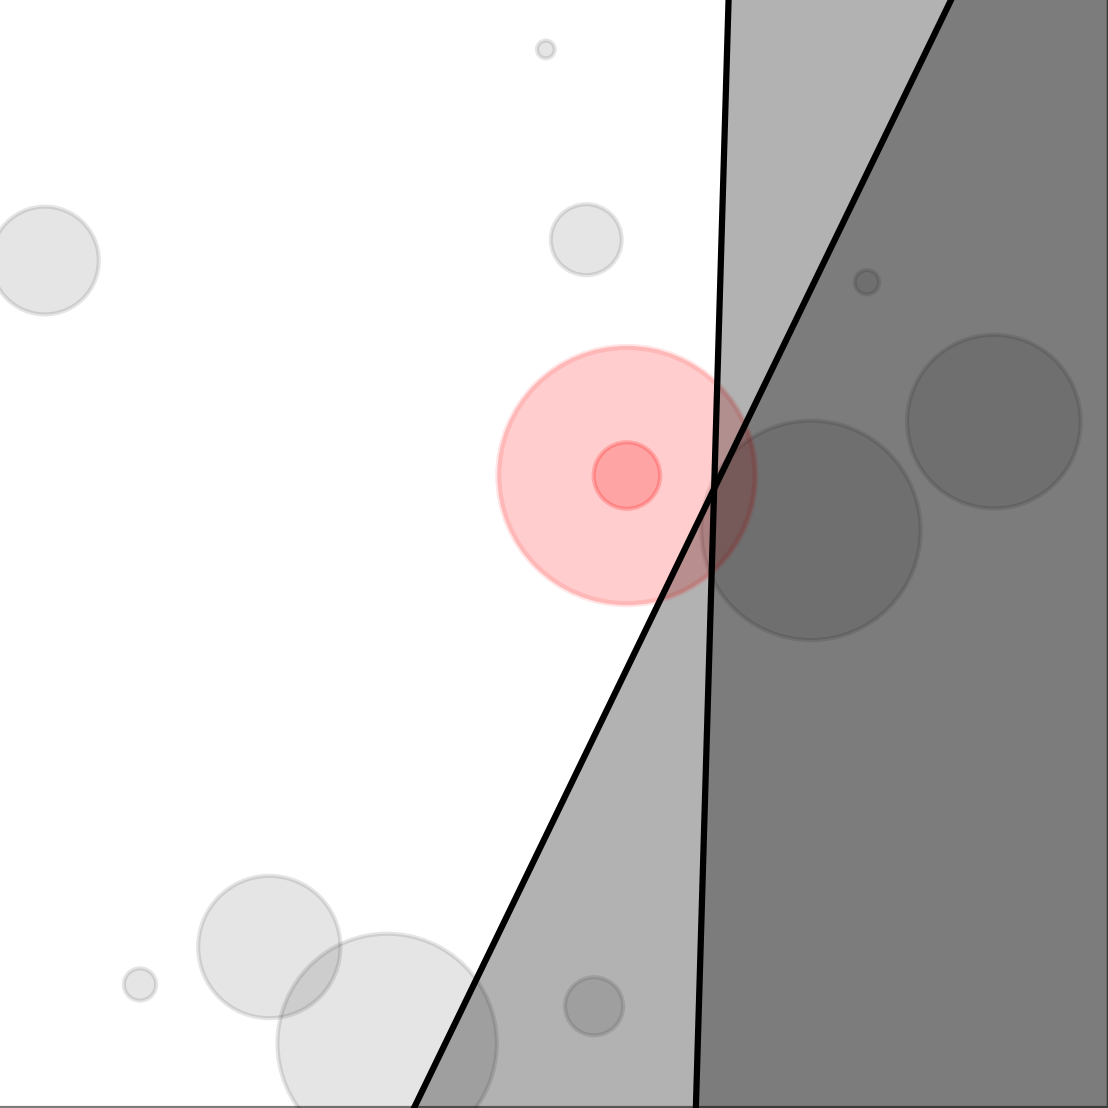
\includegraphics[width=.95\textwidth]{methods/fsd_plot_1.png}
    \vspace*{0.5em}
  \end{subfigure}%
  \begin{subfigure}{0.33\linewidth}
    \centering
    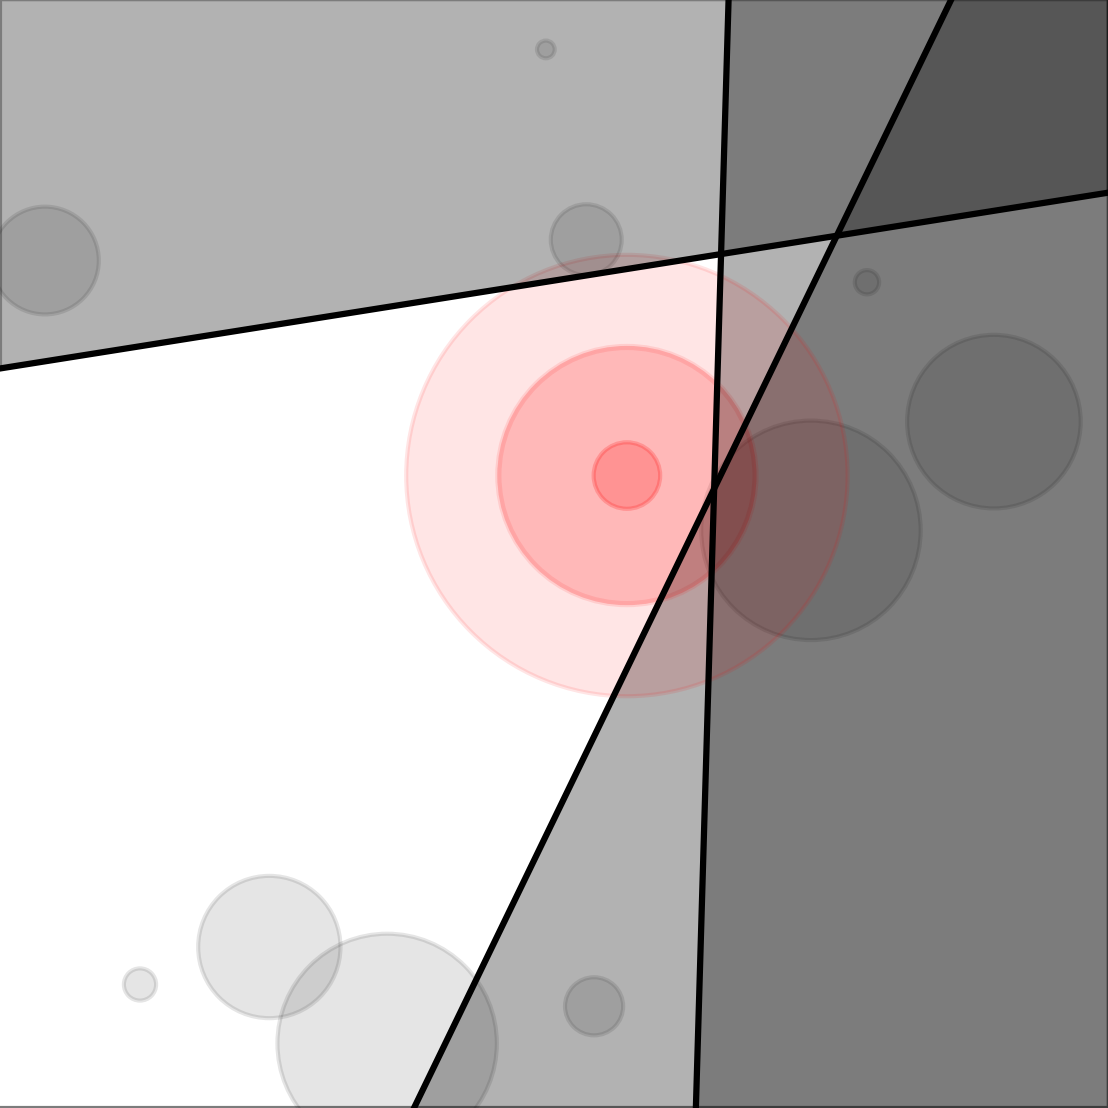
\includegraphics[width=.95\textwidth]{methods/fsd_plot_2.png}
    \vspace*{0.5em}
  \end{subfigure}
  \begin{subfigure}{0.33\linewidth}
    \centering
    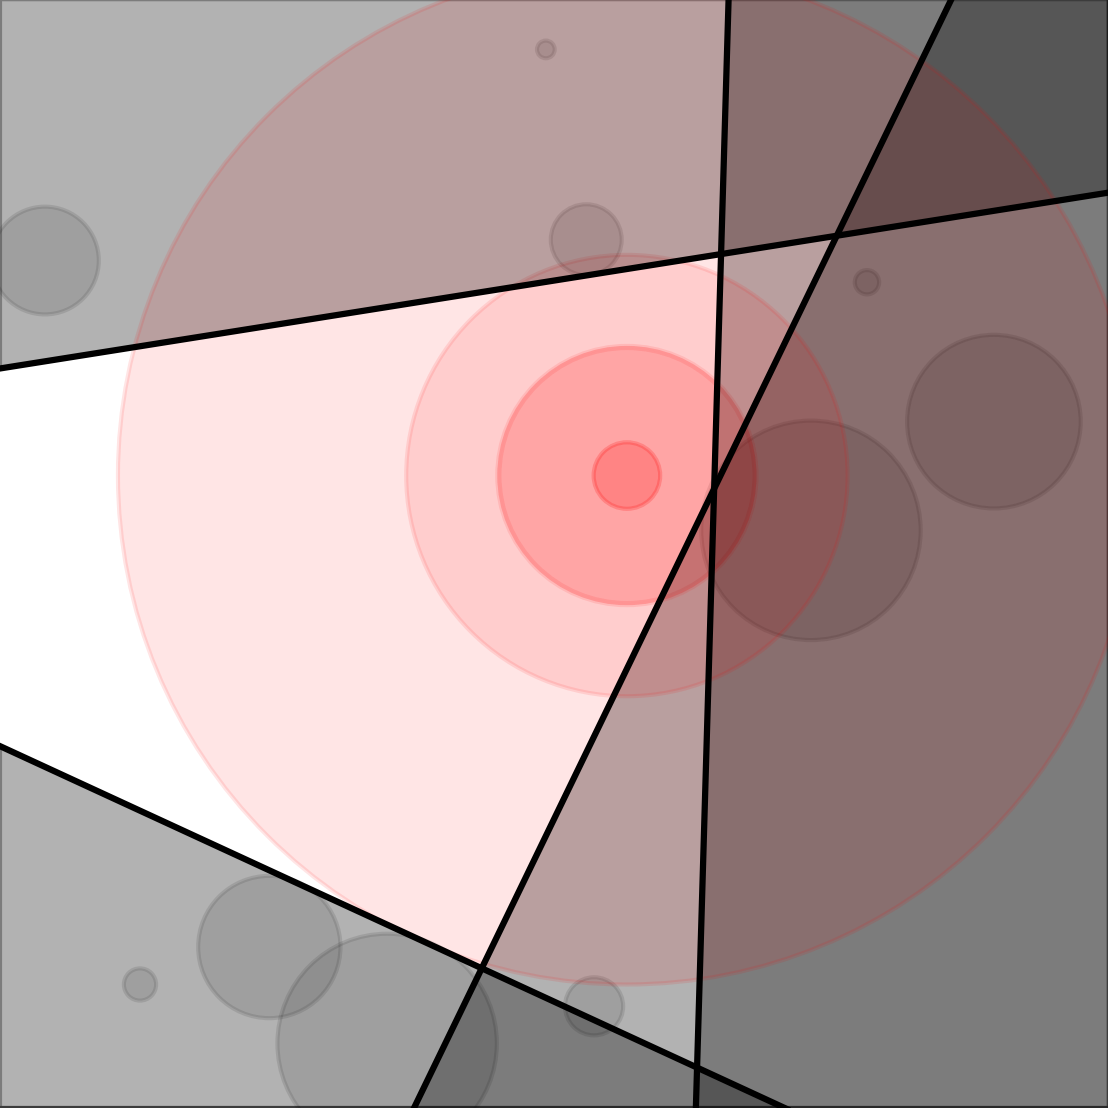
\includegraphics[width=.95\textwidth]{methods/fsd_plot_3.png}
    \vspace*{0.5em}
  \end{subfigure}%
  \begin{subfigure}{0.33\linewidth}
    \centering
    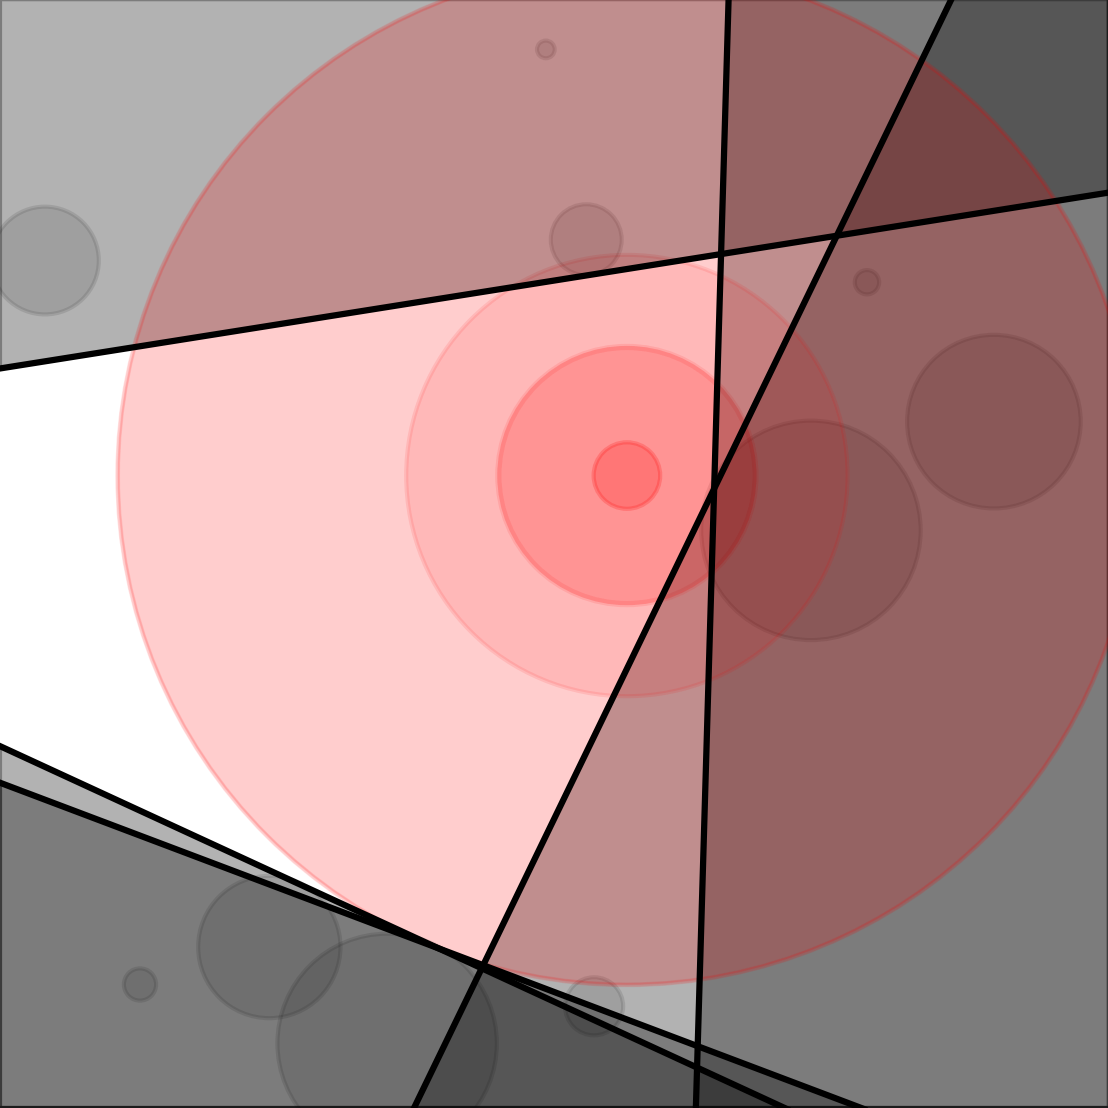
\includegraphics[width=.95\textwidth]{methods/fsd_plot_4.png}
    \vspace*{0.5em}
  \end{subfigure}%
  \begin{subfigure}{0.33\linewidth}
    \centering
    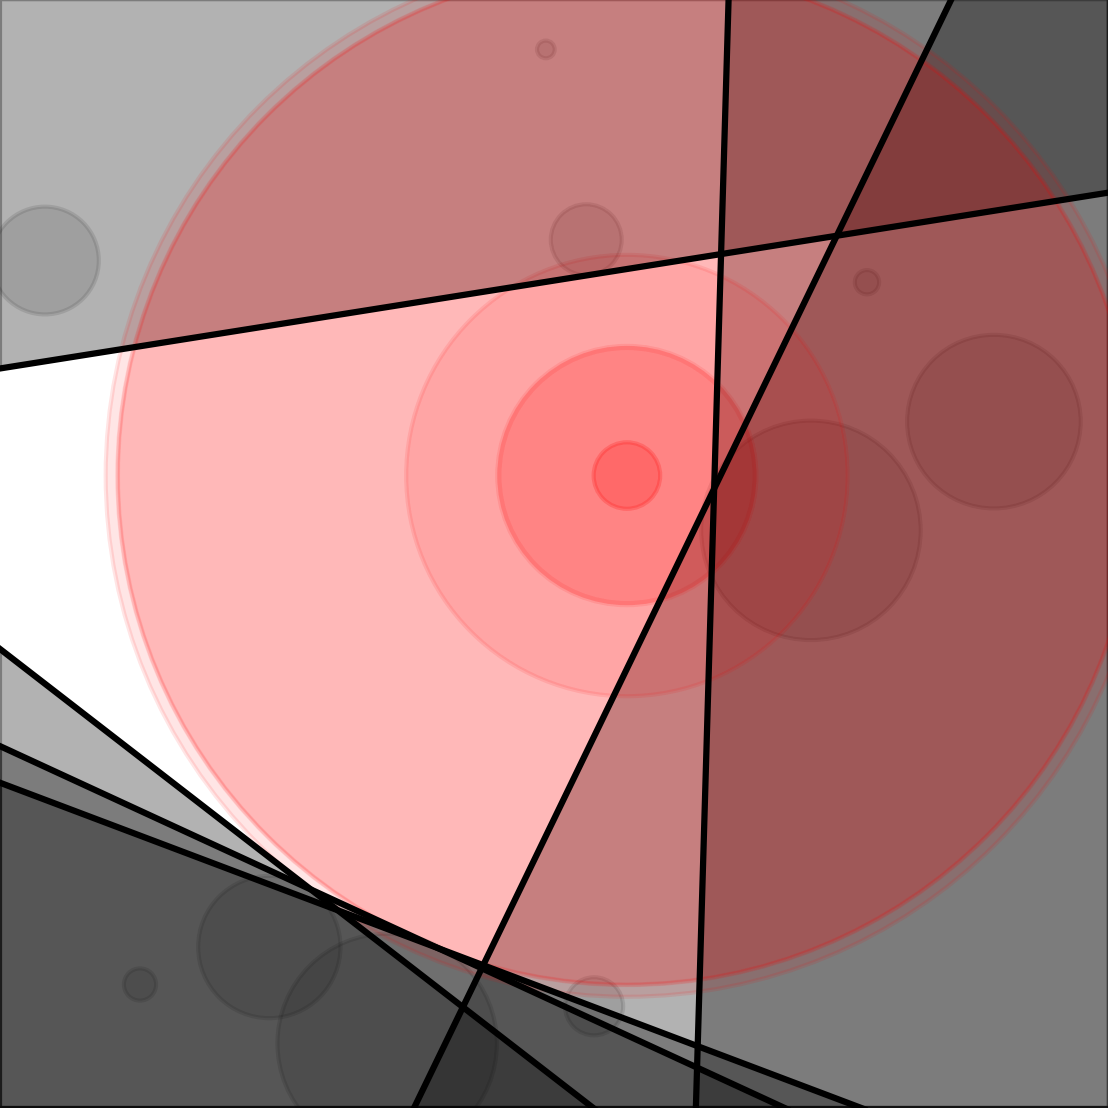
\includegraphics[width=.95\textwidth]{methods/fsd_plot_5.png}
    \vspace*{0.5em}
  \end{subfigure}%
  \caption{Iterative \acl{fsd} in 2D. The \seed{} is shown in red, obstacles in
    light gray, each \plane{} by black plane and the block workspace is shaded
    in gray. The resulting \acs{fsd} is the remaining white space.
  }%
  \label{fig:fsd}
\end{figure}

\paragraph{Representation}
Very popular in recent literature
\cite{Tordesillas2019,Liu2017a,Spahn2021} is to decompose the environment with
all its obstacles, including dynamic obstacles, into an
\ac{fsd}. Then, the
workspace in the constrained optimization is reduced to the
resulting, often convex, free space. The free space is
defined by a set of half-planes, each defined by a normal
vector \np{} and a constant \cp{}, see \cref{fig:fsd}. In
the following, we describe how the free space decomposition
can be computed given a \pointcloud{} of the environment.

The method used in this work is inspired by \cite{Liu2017a}. We define the
\seed{} for the \ac{fsd} as the \fk{} of the collision link in question. Then,
\pointcloud{} is sorted according to the euclidean distance to the \seed{}.
Starting with the closest point, a plane \plane{} defined by $\np = \point -
\seed$ and $\cp = \point$ for every $\point \in \pointcloud$. To further
speedup the process, every \point{} in \pointcloud{} that is `behind' an
existing \plane{} is removed from \pointcloud{}. The method results in set
of $\set_{\textrm{planes}} = \{\plane_i, i\in[0,n]\}$ representing the free
space around \seed{}. The algorithm is visualized in \cref{fig:fsd} for a 2D
case.

\paragraph{Integration}
We propose a method to integrate free space
decomposition into the framework of optimization \ac{fabrics}. Specifically, we
define a differentiable mapping from configuration space \Q{} to the distance
manifold between robot and each constrained plane \plane{}.
Given the \fk{} of a collision link on the robot and the radius of the
collision link, the distance to the plane \plane{} defined by its normal
\np{} and the constant \cp{}, the distance is computed as:
\begin{equation}
  \map({\plane,\fk,\rl}) = \frac{\np^T\fk + \cp}{\norm{\np}} - \rl
  \label{eq:point_plane_distance}.
\end{equation}
In contrast to \acp{sdf}, the gradients, \J{} and \Jdot{}, can be
computed analytically as a function of \q{}, \np{} and \cp{}.



\subsection{Raw sensor data}
\label{sub:raw_sensor_data}

\paragraph{Representation}
For the sake of completeness, we also include the usage of
raw sensor data into the framework of \ac{fabrics}. As
pointclouds generated with either cameras or lidars are
ususally very large, the direct usage of the raw data is not
tractable for most trajectory generation methods. However,
\ac{fabrics} are computationally efficient and can handle
large amounts of constraints more easily \cite{Spahn2023}.
This is also based on the findings by
\cite{Pantic2023obstacle} where raw sensor data was used for
drone flying with \ac{rmp}.
This allows to reduce the amount of preprocessing,
limiting the amount of uncertainty and room for error in this step. Here, we
explain how raw lidar sensor data can be utilized with \ac{fabrics}.
The same approach can be used to directly integrate pointclouds or occupancy
grids.

\paragraph{Integration}
We assume that a sensor outputs a set of
$n_{\textrm{points}}$ points \pointcloud{} in the robot`s
workspace. We integrate this data directly into \ac{fabrics}
by placing a virtual, spherical obstacle at each $\point \in
\pointcloud$. The radius of these obstacles must be chosen
to reflect the resolution of the point cloud.
